\documentclass[french]{beamer}
\usetheme[secheader]{Boadilla}
\usecolortheme[named=orange]{structure}
\usepackage[utf8]{inputenc}
\usepackage[T1]{fontenc}
\usepackage{times}
\usefonttheme{serif}
\usepackage{xkeyval}
\usepackage{todonotes}
\usepackage{amsmath,amsfonts,amssymb,amsthm}
\usepackage[acronym,toc,symbols]{glossaries}



%%%%%%%%%%%%%%%%%%%%%%%%%%%%
% Paper dependent stuff    %
%%%%%%%%%%%%%%%%%%%%%%%%%%%%


\newcommand{\ov}{\overline}
\newcommand{\oa}{\ov{a}}
%\newcommand{\oQ}{\ov{Q}}
%\newcommand{\oR}{\ov{R}}
\newcommand{\ox}{\ov{x}}
\newcommand{\oz}{\ov{z}}
\newcommand{\oy}{\ov{y}}
\newcommand{\os}{\ov{s}}
%\newcommand{\or}{\ov{r}}
%\newcommand{\ocS}{\ov{\cS}}
\newcommand{\ocF}{\ov{\cF}}
%\newcommand{\augmentedtransition}{\ov{\transition}
%\newcommand{\ocA}{\ov{\cA}}

%%%%%%%%%%%%%%%%%%%%%%%%%%%%rans
% Aesthetics               %
% over-underline, hat, bold%
%%%%%%%%%%%%%%%%%%%%%%%%%%%%

\newcommand{\eps}{\varepsilon}
\newcommand{\vareps}{\varepsilon}
\renewcommand{\epsilon}{\varepsilon}
%\renewcommand{\hat}{\widehat}
\renewcommand{\tilde}{\widetilde}
\renewcommand{\bar}{\overline}

\newcommand*{\MyDef}{\mathrm{\scriptscriptstyle def}}
\newcommand*{\eqdefU}{\ensuremath{\mathop{\overset{\MyDef}{=}}}}% Unscaled version
\newcommand*{\eqdef}{\mathop{\overset{\MyDef}{\resizebox{\widthof{\eqdefU}}{\heightof{=}}{=}}}}


\def\:#1{\protect \ifmmode {\mathbf{#1}} \else {\textbf{#1}} \fi}
\newcommand{\CommaBin}{\mathbin{\raisebox{0.5ex}{,}}}

\newcommand{\wt}[1]{\widetilde{#1}}
\newcommand{\wh}[1]{\widehat{#1}}
\newcommand{\wo}[1]{\overline{#1}}
\newcommand{\wb}[1]{\overline{#1}}

% bf and bm missing due to conflict!!
\newcommand{\bsym}[1]{\mathbf{#1}}
\newcommand{\bzero}{\mathbf{0}}
\newcommand{\ba}{\mathbf{a}}
\newcommand{\bb}{\mathbf{b}}
\newcommand{\bc}{\mathbf{c}}
\newcommand{\bd}{\mathbf{d}}
\newcommand{\be}{\mathbf{e}}
\newcommand{\bg}{\mathbf{g}}
\newcommand{\bh}{\mathbf{h}}
\newcommand{\bi}{\mathbf{i}}
\newcommand{\bj}{\mathbf{j}}
\newcommand{\bk}{\mathbf{k}}
\newcommand{\bl}{\mathbf{l}}
\newcommand{\bn}{\mathbf{n}}
%\newcommand{\bo}{\mathbf{o}}
\newcommand{\bp}{\mathbf{p}}
\newcommand{\bq}{\mathbf{q}}
\newcommand{\br}{\mathbf{r}}
\newcommand{\bs}{\mathbf{s}}
\newcommand{\bt}{\mathbf{t}}
\newcommand{\bu}{\mathbf{u}}
\newcommand{\bv}{\mathbf{v}}
\newcommand{\bw}{\mathbf{w}}
\newcommand{\bx}{\mathbf{x}}
\newcommand{\by}{\mathbf{y}}
\newcommand{\bz}{\mathbf{z}}

\newcommand{\bA}{\mathbf{A}}
\newcommand{\bB}{\mathbf{B}}
\newcommand{\bC}{\mathbf{C}}
\newcommand{\bD}{\mathbf{D}}
\newcommand{\bE}{\mathbf{E}}
\newcommand{\bF}{\mathbf{F}}
\newcommand{\bG}{\mathbf{G}}
\newcommand{\bH}{\mathbf{H}}
\newcommand{\bI}{\mathbf{I}}
\newcommand{\bJ}{\mathbf{J}}
\newcommand{\bK}{\mathbf{K}}
\newcommand{\bL}{\mathbf{L}}
\newcommand{\bM}{\mathbf{M}}
\newcommand{\bN}{\mathbf{N}}
\newcommand{\bO}{\mathbf{O}}
\newcommand{\bP}{\mathbf{P}}
\newcommand{\bQ}{\mathbf{Q}}
\newcommand{\bR}{\mathbf{R}}
\newcommand{\bS}{\mathbf{S}}
\newcommand{\bT}{\mathbf{T}}
\newcommand{\bU}{\mathbf{U}}
\newcommand{\bV}{\mathbf{V}}
\newcommand{\bW}{\mathbf{W}}
\newcommand{\bX}{\mathbf{X}}
\newcommand{\bY}{\mathbf{Y}}
\newcommand{\bZ}{\mathbf{Z}}

% calligraphic
\newcommand{\cf}{\mathcal{f}}
%\newcommand{\cA}{\mathcal{A}}
\newcommand{\cB}{\mathcal{B}}
\newcommand{\cC}{\mathcal{C}}
%\newcommand{\cD}{\mathcal{D}}
\newcommand{\cE}{\mathcal{E}}
\newcommand{\cF}{\mathcal{F}}
\newcommand{\cG}{\mathcal{G}}
\newcommand{\cH}{\mathcal{H}}
\newcommand{\cI}{\mathcal{I}}
\newcommand{\cJ}{\mathcal{J}}
\newcommand{\cL}{\mathcal{L}}
%\newcommand{\cM}{\mathcal{M}}
\newcommand{\cN}{\mathcal{N}}
\newcommand{\cO}{\mathcal{O}}
\newcommand{\cP}{\mathcal{P}}
\newcommand{\cQ}{\mathcal{Q}}
%\newcommand{\cR}{\mathcal{R}}
%\newcommand{\cS}{\mathcal{S}}
\newcommand{\cT}{\mathcal{T}}
%\newcommand{\cU}{\mathcal{U}}
\newcommand{\cV}{\mathcal{V}}
\newcommand{\cW}{\mathcal{W}}
\newcommand{\cX}{\mathcal{X}}
\newcommand{\cY}{\mathcal{Y}}
\newcommand{\cZ}{\mathcal{Z}}

\newcommand{\rf}{\mathscr{f}}
\newcommand{\rA}{\mathscr{A}}
\newcommand{\rB}{\mathscr{B}}
\newcommand{\rC}{\mathscr{C}}
\newcommand{\rD}{\mathscr{D}}
\newcommand{\rE}{\mathscr{E}}
\newcommand{\rF}{\mathscr{F}}
\newcommand{\rG}{\mathscr{G}}
\newcommand{\rH}{\mathscr{H}}
\newcommand{\rI}{\mathscr{I}}
\newcommand{\rJ}{\mathscr{J}}
\newcommand{\rK}{\mathscr{K}}
\newcommand{\rL}{\mathscr{L}}
\newcommand{\rM}{\mathscr{M}}
\newcommand{\rN}{\mathscr{N}}
\newcommand{\rO}{\mathscr{O}}
\newcommand{\rP}{\mathscr{P}}
\newcommand{\rQ}{\mathscr{Q}}
\newcommand{\rR}{\mathscr{R}}
\newcommand{\rS}{\mathscr{S}}
\newcommand{\rT}{\mathscr{T}}
\newcommand{\rU}{\mathscr{U}}
\newcommand{\rV}{\mathscr{V}}
\newcommand{\rW}{\mathscr{W}}
\newcommand{\rX}{\mathscr{X}}
\newcommand{\rY}{\mathscr{Y}}
\newcommand{\rZ}{\mathscr{Z}}

\newcommand{\bbf}{\mathbb{f}}
\newcommand{\bbA}{\mathbb{A}}
\newcommand{\bbB}{\mathbb{B}}
\newcommand{\bbC}{\mathbb{C}}
\newcommand{\bbD}{\mathbb{D}}
\newcommand{\bbE}{\mathbb{E}}
\newcommand{\bbF}{\mathbb{F}}
\newcommand{\bbG}{\mathbb{G}}
\newcommand{\bbH}{\mathbb{H}}
\newcommand{\bbI}{\mathbb{I}}
\newcommand{\bbJ}{\mathbb{J}}
\newcommand{\bbK}{\mathbb{K}}
\newcommand{\bbL}{\mathbb{L}}
\newcommand{\bbM}{\mathbb{M}}
\newcommand{\bbN}{\mathbb{N}}
\newcommand{\bbO}{\mathbb{O}}
\newcommand{\bbP}{\mathbb{P}}
\newcommand{\bbQ}{\mathbb{Q}}
\newcommand{\bbR}{\mathbb{R}}
\newcommand{\bbS}{\mathbb{S}}
\newcommand{\bbT}{\mathbb{T}}
\newcommand{\bbU}{\mathbb{U}}
\newcommand{\bbV}{\mathbb{V}}
\newcommand{\bbW}{\mathbb{W}}
\newcommand{\bbX}{\mathbb{X}}
\newcommand{\bbY}{\mathbb{Y}}
\newcommand{\bbZ}{\mathbb{Z}}


%%%%%%%%%%%%%%%%%%%%%%%%%%%%
% Math jargon              %
%%%%%%%%%%%%%%%%%%%%%%%%%%%%
\newcommand{\wrt}{w.r.t.\xspace}
\newcommand{\defeq}{\stackrel{\mathclap{\normalfont\mbox{\scriptscriptstyle def}}}{=}}
\newcommand{\maxund}[1]{\max\limits_{#1}}
\newcommand{\supund}[1]{\text{sup}\limits_{#1}}
\newcommand{\minund}[1]{\min\limits_{#1}}
\renewcommand{\epsilon}{\varepsilon}
\newcommand{\bigotime}{\mathcal{O}}


\DeclareMathOperator*{\argmin}{arg\,min} 
\DeclareMathOperator*{\argmax}{arg\,max} 
\DeclareMathOperator*{\cupdot}{\mathbin{\mathaccent\cdot\cup}}

%%%%%%%%%%%%%%%%%%%%%%%%%%%%
% Matrix operators         %
%%%%%%%%%%%%%%%%%%%%%%%%%%%%
\newcommand{\transp}{\mathsf{\scriptscriptstyle T}}

%%%%%%%%%%%%%%%%%%%%%%%%%%%%
% Statistic operators      %
%%%%%%%%%%%%%%%%%%%%%%%%%%%%
\newcommand{\probability}[1]{\mathbb{P}\left(#1\right)}
\newcommand{\probdist}{Pr}
\DeclareMathOperator*{\expectedvalue}{\mathbb{E}}
\DeclareMathOperator*{\variance}{\text{Var}}
\newcommand{\expectedvalueover}[1]{\expectedvalue\limits_{#1}}
\newcommand{\condbar}{\;\middle|\;}
\newcommand{\gaussdistr}{\mathcal{N}}
\newcommand{\uniformdistr}{\mathcal{U}}
\newcommand{\bernoullidist}{\mathcal{B}}

%%%%%%%%%%%%%%%%%%%%%%%%%%%%
% Algebraic Sets           %
%%%%%%%%%%%%%%%%%%%%%%%%%%%%
\newcommand{\Real}{\mathbb{R}}
\newcommand{\Natural}{\mathbb{N}}
\newcommand{\statespace}{\mathcal{X}}
\newcommand{\funcspace}{\mathcal{F}}
\newcommand{\dynaspace}{\mathcal{T}}


%\newtheorem{theorem}{Theorem}
%\newtheorem{definition}{Definition}
%\newtheorem{lemma}{Lemma}
%\newtheorem{proposition}{Proposition}
%\newtheorem{remark}{Remark}
%\newtheorem{property}{Property}
%\newtheorem{assumption}{Assumption}
%\newtheorem{conjecture}{Conjecture}


%\newacronym{RL}{RL}{Reinforcement Learning}
\newacronym[longplural={Markov Decision Processes}]{MDP}{MDP}{Markov Decision Process}
\newacronym[longplural={Partially Observable Markov Decision Processes}]{POMDP}{POMDP}{Partially Observable Markov Decision Process}
\newacronym{SRS}{SRS}{Speech Recognition Score}
\newacronym{SER}{SER}{Sentence Error Rate}
\newacronym{DBN}{DBN}{Deep Belief Network}
\newacronym{VI}{VI}{Value Iteration}
\newacronym{PI}{PI}{Policy Iteration}
\newacronym{SGD}{SGD}{Stochastic Gradient Descent}
\newacronym{iid}{iid}{independent and identically distributed}
\newacronym{RBM}{RBM}{Restricted Boltzmann Machine}
\newacronym{MAML}{MAML}{Model-Agnostic Meta-Learning}
%\newacronym{MOBA}{MOBA}{Multiplayer Online Battle Arena}
%\newacronym{UAV}{UAV}{Unmanned Aerial Vehicule}
%\newacronym{RTS}{RTS}{Real Time Strategy}
\newacronym{GD}{GD}{Gradient Descent}
\newacronym{LS}{LS}{Least Squares}
\newacronym{TD}{TD}{Temporal Difference}
\newacronym{FTQ}{FTQ}{Fitted-$Q$}
\newacronym{BFTQ}{BFTQ}{Budgeted Fitted-$Q$}
\newacronym{DM}{DM}{Dialogue Manager}
\newacronym{DQN}{DQN}{Deep $Q$-learning}
\newacronym{A3C}{A3C}{Asynchronous Actor-Critic Agents}
\newacronym{DRL}{DRL}{Deep Reinforcement Learning}
\newacronym{FVI}{FVI}{Fitted-Value-Iteration}
\newacronym{AVI}{AVI}{Approximate Value Iteration}
\newacronym{API}{API}{Approximate Policy Iteration}
\newacronym{PG}{PG}{Policy Gradient}
\newacronym{AC}{AC}{Actor Critic}
\newacronym{TTS}{TTS}{Text To Speech}
\newacronym{GAN}{GAN}{Generative Adversarial Network}
\newacronym{DOD}{DOD}{Department of Defense}
\newacronym{DARPA}{DARPA}{Defense Advanced Research Projects Agency}
\newacronym{HMM}{HMM}{Hidden Markov Model}
\newacronym{TL}{TL}{Transfer Learning}
\newacronym{SL}{SL}{Supervised Learning}
\newacronym{GP}{GP}{Gaussian Process}
\newacronym{SDS}{SDS}{Spoken Dialogue System}
\newacronym{NN}{NN}{Neural Network}
\newacronym{CNN}{CNN}{Convolutional Neural Network}
\newacronym[longplural={Dialogue Systems}]{DS}{DS}{Dialogue System}
%\newacronym{BUDS}{BUDS}{The Bayesian Update of Dialogue State}
\newacronym{DST}{DST}{Dialogue State Tracking}
\newacronym{DSTC}{DSTC}{Dialogue State Tracking Challenge}
\newacronym{LSPI}{LSPI}{Least Squares Policy Iteration}
\newacronym{ASR}{ASR}{Automatic Speech Recognition}
\newacronym{NDG}{NDG}{Negociation Dialogue Game}
\newacronym{UCB}{UCB}{Upper Bound Confidence}
\newacronym{ML}{ML}{Machine Learning}
\newacronym{AI}{A.I.}{Artificial Intelligence}
\newacronym{GPU}{GPU}{Graphics Processing Unit}
\newacronym{CPU}{CPU}{Central Processing Unit}
\newacronym{RNN}{RNN}{Recurrent Neural Networks}
\newacronym{LSTM}{LSTM}{Long Short-Term Memory}
\newacronym{NLG}{NLG}{Natural Language Generator}
\newacronym{NLU}{NLU}{Natural Language Understanding}
\newacronym{MIT}{MIT}{Massachusset Institute of Technology}
\newacronym[longplural={Dialogue Policies}]{DP}{DP}{Dialogue Policy}
\newacronym{MAB}{MAB}{Multi-Armed Bandit}
\newacronym{ACER}{ACER}{Actor Critic Experience Replay}
\newacronym{ER}{ER}{Experience Replay}
\newacronym{BMDP}{BMDP}{Budgeted Markov Decision Process}
\newacronym{CMDP}{CMDP}{Constrainted Markov Decision Process}
\newacronym{AGI}{AGI}{Artificial General Intelligence}
\newacronym{BVI}{BVI}{Budgeted Value Iteration}
\newacronym{REINFORCE}{REINFORCE}{REINFORCE}
\newacronym{kNN}{$k$NN}{$k$ Nearest Neighbours}
\newacronym{GUS}{GUS}{Genial Understander System}
\newacronym{VaR}{VaR}{Value at Risk}
\newacronym{CVaR}{CVaR}{Conditional Value at Risk}
\newacronym{MORL}{MORL}{Multi-Objectives Reinforcement Learning}
\newacronym{SARSA}{SARSA}{State–Action–Reward–State–Action}
%\newacronym{}{}{}
%\newacronym{}{}{}
\newcommand{\ftq}{\textrm{\textsc{FTQ}}\xspace}
\newcommand{\bftq}{\textrm{\textsc{BFTQ}}\xspace}


\newcommand{\Q}{Q}
\newcommand{\V}{V}
\newcommand{\mubot}{\mu_{\bot}}
\newcommand{\mutop}{\mu_{\top}}
\newcommand{\params}{\theta}
\newcommand{\dirac}{\delta}
\newcommand{\normal}{\mathcal{N}}
\newcommand{\binomial}{\mathcal{B}}
\newcommand{\features}{\phi}
\newcommand{\maxiteration}{K}
\newcommand{\deltastoppingcriterion}{\upsilon}
\newcommand{\extrasmallvalue}{\kappa}
\newcommand{\egreedy}{\epsilon}
\newcommand{\users}{\rU}
\newcommand{\timeslot}{\tau}
\newcommand{\cooperationrate}{\varrho}
\newcommand{\T}{N}
\newcommand{\srs}{\nu}
\newcommand{\ser}{\xi}
\newcommand{\transpose}{\top}
\newcommand{\indextransition}{i}
\newcommand{\state}{s}
\newcommand{\n}{k}
\newcommand{\learningrate}{\alpha}
\newcommand{\abo}{\overline{\mathcal{T}}}
\newcommand{\bo}{\mathcal{T}}
\newcommand{\oQ}{\overline{Q}}
\newcommand{\Qr}{Q_r}
\newcommand{\Qc}{Q_c}
\newcommand{\oR}{\overline{R}}
\newcommand{\oV}{\overline{V}}
\newcommand{\Vr}{V_r}
\newcommand{\Vc}{V_c}
\newcommand{\ocS}{\overline{\mathcal{S}}}
\newcommand{\ocA}{\overline{\mathcal{A}}}
\newcommand{\cS}{\mathcal{S}}
\newcommand{\budgetspace}{\mathscr{B}}
\newcommand{\cK}{\mathcal{K}}
\newcommand{\policies}{\overline{\Pi}}
\newcommand{\cU}{\mathcal{U}}
\newcommand{\cA}{\mathcal{A}}
\newcommand{\augmentedtransition}{\overline{P}}
\newcommand{\cD}{\mathcal{D}}
\newcommand{\reward}{R}
\newcommand{\augmentedreward}{\overline{R}}
\newcommand{\constraint}{C}
\newcommand{\transition}{P}
\newcommand{\return}{G}
\newcommand{\constraintreturn}{G_c}
\newcommand{\augmentedreturn}{\overline{G}}
\newcommand{\cM}{\mathcal{M}}
\newcommand{\policy}{\pi}
\newcommand{\budgetedpolicy}{\overline{\pi}}
\newcommand{\optimalpolicy}{\pi^*}
\newcommand{\optimalbudgetedpolicy}{\overline{\pi}^*}
\newcommand{\discountfactor}{\gamma}
\newcommand{\budgetaction}{\beta_a}
\newcommand{\nextbudget}{\beta'}
\newcommand{\budget}{\beta}
\newcommand{\projection}{\Xi}
\newcommand{\augmentedprojection}{\overline{\Xi}}

\presetkeys{todonotes}{inline}{}
\title[TITLE]{Apprentissage par renforcement pour l'optimisation des systèmes de dialogue via l'adaptation à l'utilisateur.}
\subtitle{Soutenance de thèse.}
\author{Nicolas Carrara}
\institute[ULille]{Université de Lille}
\date{Le 18 Décembre 2019}

\setbeamertemplate{footline}{%
\hfill%
\usebeamercolor[fg]{page number in head/foot}%
\usebeamerfont{page number in head/foot}%
\insertframenumber%
%\,/\,\inserttotalframenumber
\kern1em\vskip2pt%
}

\beamertemplatenavigationsymbolsempty

\begin{document}

    \begin{frame}
        \maketitle
        \centering
    \end{frame}

    \section{Introduction}

    \begin{frame}{Les sytèmes de dialogues}

        \todo{Schéma avec c'est quoi un système de dialogue}

    \end{frame}

    \begin{frame}{Trois types d'applications}

        \begin{itemize}
            \item Discussion social sans but précis.
            \item Question-Réponse
            \item Dialogues orientés tâches.
        \end{itemize}

        %C'est surtout la troisième problématique qui nous interesse.
        \todo{mettre en gras ou avant la troisème problématique}

    \end{frame}

    \begin{frame}{Personalisation}

        % avec l'essort du smartphone/car/etc
        De plus en plus de systèmes deviennent personnels

        \begin{itemize}
            \item Assistants personnels % par définition personnels
            \item Maisons connectées % parler à l'enfant, les parents etc (les enfants sont moins succeptible de demander certain choses etc)
            \item Voitures connectées
            % handfree gps etc
        \end{itemize}

        \todo{TODO mettre deux trois images ici}

    \end{frame}

    \begin{frame}{Problématique}

        On pourrait discriminer deux types de personalisations

        \begin{itemize}
            \item Adaptation aux habitudes de la personne.
            % les rdv sont plutot le dimanche, le medecin s'appelle X, la personne habide dans un coin avec certains restaurant
            \item Adaptation au type de personne.
            % personne agée, enfant, dyslesique, culture (red good chine, red wrong europe) etc
        \end{itemize}

        %C'est surtout la deuxième problématique qui nous interesse.
        \todo{mettre en gras ou avant la deuxième problématique}

        \begin{alertblock}{Problématique}
            Comment s'adapter sans a priori?
        \end{alertblock}

    \end{frame}

    \begin{frame}{Pistes de recherche}

        %On va explorer
        Deux directions, toutes deux exploitant l'apprentissage par transfert.

        \begin{itemize}
            \item Approche classique, avec l'utilisation d'outils existants et leur mise à l'echelle.
            \item Approche plus conservatrice, en mettant en avant la notion de risque dans la conversation.
        \end{itemize}


        %Mais concrétement,
        Comment fonctionne un système de dialogue ?

    \end{frame}

    \section{Systèmes de dialogue orientées tâches}



    \subsection{Pipeline}


    \begin{frame}{L'exemple du Slot-Filling}

        Expliquer le slot filling

        Faire la transition sur comment modéliser le processus

    \end{frame}

    \foreach \n in {1,2,3,4,5,6,7}{
    \begin{frame}{Le processus (\n/7)}
        \begin{figure}
            \centering
            %%\vspace{-1.5em}
            \includegraphics[scale=0.7,page=1]{img/pipeline\n}
        \end{figure}
    \end{frame}
    }

    \foreach \n in {1,2}{
    \begin{frame}{Un problème de décision séquentielle (\n/2)}
        \begin{figure}
            \centering
            %%\vspace{-1.5em}
            \includegraphics[scale=0.55,page=1]{img/pipeline-dp\n}
        \end{figure}
    \end{frame}
    }




    \begin{frame}
        %On réduit le problème à cette échange
        \begin{figure}
            \centering
            %%\vspace{-1.5em}
            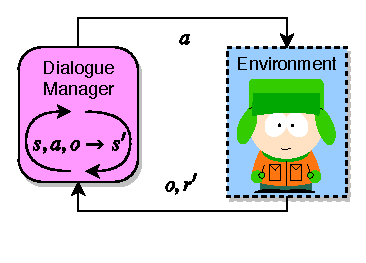
\includegraphics[scale=1.0,page=1]{../sources/dm-rl/rl-pipeline}
        \end{figure}
        \todo{dire a quoi correspond chaque etat, par rapport au slide de slot filling}

        \begin{alertblock}{}
            Comment décider l'action à choisir en fonction de l'état courant ?
        \end{alertblock}
    \end{frame}

    \subsection{RL}
    \begin{frame}

        A MDP is a tuple $\langle{}\cS,\cA,\reward,\transition,\discountfactor\rangle{}$ where:
        \begin{itemize}
            \item  $\cS$ is the state set,
            \item  $\cA$ is the action set,
            \item $\reward\in\Real^{\cS \times \cA}$ is the reward function,
            \item $\transition\in \cM(\cS)^{\cS \times \cA}$ is the transition kernel; $\cM(\cX)$ denotes the probability measure over a set $\cX$.
            \item $\discountfactor$ is the discount factor.
        \end{itemize}

    \end{frame}

    \begin{frame}
        policy

        Q function

        Bellman control equation

    \end{frame}

    \begin{frame}

        continuous AND unkwon env

        FTQ

        -> unknown env we need sample, if we don't know the user, we don't have samples -> transfer learning

    \end{frame}

    \subsection{TL}
    \begin{frame}

    \end{frame}

    \section{Passage à l'échelle de l'apprentissage par transfert}

    \subsection{Sigdial}

    \begin{frame}
        Sigdial
    \end{frame}

    \subsection{Transfert continu}

    \begin{frame}

        TDQN

    \end{frame}

    \subsection{}

    \begin{frame}
        Le plus important dans un nouveau systèmes, c'est de garder l'user. Alors, au lieu d'optimiser, pourquoi ne pas focus sur le fait de pas le faire fuir ?
    \end{frame}

    \section{Apprentissage par transfert sécurisé}

    \subsection{epsilon safe}
    \begin{frame}

        explore
        exploite
        pi safe
        rajoute une info supplementaire (safery) lié intimement à la reussite, et peut donc guider l'apprentissage
        eviter les endroits trop unsafe pour garder l'user
    \end{frame}

    \begin{frame}
        Les results sont pas probants.
        Pourquoi ?
        l'environement est trop simple
        cette information n'est pas exploiter comme il faut
        single reward suffer from TOO safe TOO unsafe
        peut etre quand dans ce cas c'était trop unsafe
        comment construit des politiques safe sans end up with extreme behavious ? -> BFTQ
    \end{frame}

    \subsection{Créer un système précautionneux, mais pas trop.}

    \begin{frame}

        BFTQ

    \end{frame}

    \section{Conclusion}
    \begin{frame}
    \end{frame}

    \begin{frame}
        \begin{block}{Block}
            Standard beamer block
        \end{block}
        \begin{alertblock}{Block}
            Alert block
        \end{alertblock}
        \begin{exampleblock}{Block}
            Example block
        \end{exampleblock}
    \end{frame}


\end{document}

